% =====================================================================
%  Introduccion (2 diapositivas, Guia 2.1: sin sistema ni metodo particular)
% =====================================================================

% SLIDE intro_real | V:A | T:25
\begin{frame}{Evacuación de una sala}
  \begin{columns}[c]
    \begin{column}{0.56\textwidth}
      \begin{itemize}
        \item Sala cuadrada con una única puerta estrecha.
        \item Lejos de la puerta: zona diluida, movimiento casi rectilíneo, contactos raros.
        \item En la puerta: cuello de botella, contactos continuos.
        \item Régimen mixto: contactos raros lejos de la puerta, continuos en la cola.
      \end{itemize}
    \end{column}
    \begin{column}{0.40\textwidth}
      \centering
      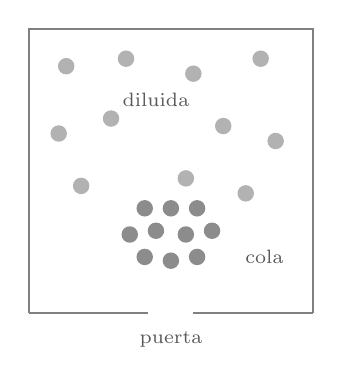
\begin{tikzpicture}[scale=0.95]
        \draw[thick,gray] (-1.9,-1.9) -- (-0.3,-1.9);
        \draw[thick,gray] (0.3,-1.9) -- (1.9,-1.9);
        \draw[thick,gray] (-1.9,-1.9) -- (-1.9,1.9) -- (1.9,1.9) -- (1.9,-1.9);
        \foreach \x/\y in {-1.4/1.4, -0.6/1.5, 0.3/1.3, 1.2/1.5, -1.5/0.5, -0.8/0.7,
                           0.7/0.6, 1.4/0.4, -1.2/-0.2, 0.2/-0.1, 1.0/-0.3}
          \fill[gray!60] (\x,\y) circle (0.11);
        \foreach \x/\y in {-0.35/-1.15, 0.0/-1.2, 0.35/-1.15, -0.55/-0.85, -0.2/-0.8,
                           0.2/-0.85, 0.55/-0.8, -0.35/-0.5, 0.0/-0.5, 0.35/-0.5}
          \fill[gray!90] (\x,\y) circle (0.11);
        \node[font=\scriptsize,gray!70!black] at (0,-2.25) {puerta};
        \node[font=\scriptsize,gray!70!black] at (-0.2,0.95) {diluida};
        \node[font=\scriptsize,gray!70!black] at (1.25,-1.15) {cola};
      \end{tikzpicture}
    \end{column}
  \end{columns}
\end{frame}

% SLIDE intro_sfm | V:A | T:40
\begin{frame}{Modelo de fuerza social, solo contacto}
  \small
  \[
    m\,\dot{\vect v}_i = m\,\frac{v_d\,\hat{\vect e}_i-\vect v_i}{\tau}
      + \sum_{j}\vect F^c_{ij} + \sum_{w}\vect F^c_{iw}
  \]
  \[
    \vect F^c_{ij} = k\,g(\xi_{ij})\,\hat{\vect n}_{ij}
      + \kappa\,g(\xi_{ij})\,(\Delta\vect v_{ij}\cdot\hat{\vect t}_{ij})\,\hat{\vect t}_{ij},
    \qquad \xi_{ij}=r_i+r_j-d_{ij},\quad g(x)=\max(x,0)
  \]
  \begin{itemize}
    \item Deseo: velocidad $v_d$ hacia el objetivo ($\hat{\vect e}_i$) con tiempo de relajación $\tau$.
    \item Contacto: resorte normal (rigidez $k$) y fricción tangencial ($\kappa$) sobre la
      superposición $\xi_{ij}$; sin fuerza social.
    \item Paredes y bordes de la puerta: el mismo contacto con un agente de radio $0$.
  \end{itemize}
  \vfill
  {\scriptsize (Helbing, Farkas y Vicsek, Nature, 2000)}
\end{frame}
